%%%%%%%%%%%%%%%%%%%%%%%%%%%%%%%%%%%%%%%%%%%%%%%%%%%%%%%%%%%%%%%%%%%%%%%%%%%%%%%%
% TUM-Vorlage: Präsentation
%%%%%%%%%%%%%%%%%%%%%%%%%%%%%%%%%%%%%%%%%%%%%%%%%%%%%%%%%%%%%%%%%%%%%%%%%%%%%%%%
%
% Rechteinhaber:
%     Technische Universität München
%     https://www.tum.de
%
% Gestaltung:
%     ediundsepp Gestaltungsgesellschaft, München
%     http://www.ediundsepp.de
%
% Technische Umsetzung:
%     eWorks GmbH, Frankfurt am Main
%     http://www.eworks.de
%
%%%%%%%%%%%%%%%%%%%%%%%%%%%%%%%%%%%%%%%%%%%%%%%%%%%%%%%%%%%%%%%%%%%%%%%%%%%%%%%%


%%%%%%%%%%%%%%%%%%%%%%%%%%%%%%%%%%%%%%%%%%%%%%%%%%%%%%%%%%%%%%%%%%%%%%%%%%%%%%%%
% Zur Wahl des Seitenverhältnisses bitte einen der beiden folgenden Befehle
% auskommentieren und den ausführen lassen:
\documentclass[handout,t,aspectratio=43]{beamer}
% \documentclass[notes,t,aspectratio=43]{beamer}
\usepackage[
    orientation=landscape,
    size=custom,
    width=25.4,
    height=19.05,
    scale=0.7 % erzeugt 16pt Schriftgröße
]{beamerposter}

% Display Notes for pympress
\usepackage{pgfpages}
% \setbeameroption{show notes on second screen=right}
\setbeamertemplate{note page}[plain]
\setbeamerfont{note page}{size=\Large}

\newcommand{\PraesentationSchriftgroesseSehrGross}{\fontsize{30}{45}}
\newcommand{\PraesentationSchriftgroesseGross}{\fontsize{22}{33}}
\newcommand{\PraesentationSchriftgroesseNormal}{\fontsize{16}{29}}
\newcommand{\PraesentationSchriftgroesseKlein}{\fontsize{12}{18}}
\newcommand{\PraesentationSchriftgroesseDreizeiler}{\fontsize{7}{10}}
\newcommand{\PraesentationSchriftgroesseAufzaehlungszeichen}{\fontsize{10}{8}}

\newcommand{\PraesentationAbstandAbsatz}{22.1pt}
\newcommand{\PraesentationPositionKorrekturOben}{0cm}
\newcommand{\PraesentationBeispieleSchriftgroessen}{30 | 22 | 16 | 12}
\usepackage[utf8]{inputenc}
\usepackage[T1]{fontenc} % Zeichensatzkodierung

\usepackage{calc} % Berechnungen

\usepackage[ngerman]{babel} % Deutsche Lokalisierung
\usepackage{graphicx} % Grafiken
\usepackage[absolute, overlay]{textpos} % Positionierung

% Silbentrennung:
\usepackage{hyphenat}
%\tolerance 2414
%\hbadness 2414
%\emergencystretch 1.5em
%\hfuzz 0.3pt
%\widowpenalty=10000     % Hurenkinder
%\clubpenalty=10000      % Schusterjungen
%\vfuzz \hfuzz

% Euro-Symbol:
\usepackage[gen]{eurosym}
\DeclareUnicodeCharacter{20AC}{\euro{}}

% Schriftart Helvetica:
\usepackage[scaled]{helvet}
\renewcommand{\familydefault}{\sfdefault}

\usepackage{mathptmx} % skalierbare Formelschriften

\usepackage{tabularx}

\usepackage{multicol} % mehrspaltiger Text

\usepackage{tikz}
\usetikzlibrary{arrows, shapes, shapes.multipart, trees, positioning,
    backgrounds, fit, matrix, external, overlay-beamer-styles}

% Diagramme:
\usepackage{pgfplots}
\pgfplotsset{compat=default}

% Erweiterbare Fusszeile:
\newcommand{\PraesentationFusszeileZusatz}{}

\usepackage{bookmark} % Lesezeichen

% Unterdrückung layoutbedingter Warnungen
\usepackage[immediate]{silence}
\WarningFilter[layout]{lastpage}{Rerun to get the references right} % Gesamtseitenzahl
\WarningFilter[layout]{latex}{Label(s) may have changed.} % Referenz auf letzte Seite
\WarningFilter[layout]{pgfplots}{running in backwards compatibility mode (unsuitable tick labels; missing features).} % Labelerstellung ab Version 1.17 nicht abwärtskompatibel
\WarningFilter[layout]{latex}{There were undefined references}
\WarningFilter[layout]{latex}{Reference `PraesentationDiagramm} % Erstellung einer Legende außerhalb des Diagrammbereichs

% Debugging:
%\DeactivateWarningFilters[layout] % Unterdrückte Warnungen einschalten
\usepackage{listings}

\lstdefinelanguage{rv64}{
    morekeywords={
        addi, bne,
        a1, x0
    },
    sensitive=false
}

\definecolor{SbtComment}{RGB}{80, 80, 80}

\lstdefinelanguage{SbtIr}{
    morekeywords={
        block,
        i64, i32, i16, i8, imm,
        immediate, add,
        cjump, jump
    },
    morecomment=[l]{//},
    morecomment=[s]{/*}{*/}
}

\usepackage[verbatim]{lstfiracode}
\lstset{
    style=FiraCodeStyle, % Use predefined FiraCodeStyle
    basicstyle=\ttfamily, % Use \ttfamily for source code listings
    keywordstyle=\color{TUMBlauDunkel},
    commentstyle=\color{SbtComment}
}

 % Seitenverhältnis 16:9
%%%%%%%%%%%%%%%%%%%%%%%%%%%%%%%%%%%%%%%%%%%%%%%%%%%%%%%%%%%%%%%%%%%%%%%%%%%%%%%%


%%%%%%%%%%%%%%%%%%%%%%%%%%%%%%%%%%%%%%%%%%%%%%%%%%%%%%%%%%%%%%%%%%%%%%%%%%%%%%%%
%%%%%%%%%%%%%%%%%%%%%%%%%%%%%%%%%%%%%%%%%%%%%%%%%%%%%%%%%%%%%%%%%%%%%%%%%%%%%%%%
% TUM-Vorlage: Personenspezifische Informationen
%%%%%%%%%%%%%%%%%%%%%%%%%%%%%%%%%%%%%%%%%%%%%%%%%%%%%%%%%%%%%%%%%%%%%%%%%%%%%%%%
%
% Rechteinhaber:
%     Technische Universität München
%     https://www.tum.de
% 
% Gestaltung:
%     ediundsepp Gestaltungsgesellschaft, München
%     http://www.ediundsepp.de
% 
% Technische Umsetzung:
%     eWorks GmbH, Frankfurt am Main
%     http://www.eworks.de
%
%%%%%%%%%%%%%%%%%%%%%%%%%%%%%%%%%%%%%%%%%%%%%%%%%%%%%%%%%%%%%%%%%%%%%%%%%%%%%%%%

% Für die Person anpassen:

% Allgemein:
\newcommand{\AllgemeinGestalter}{ediundsepp Gestaltungsgesellschaft}
\newcommand{\AllgemeinErsteller}{eWorks GmbH}

% Universität:
\newcommand{\UniversitaetName}{Technische Universität München}
\newcommand{\UniversitaetAbkuerzung}{TUM}
\newcommand{\UniversitaetWebseite}{www.tum.de}
\newcommand{\UniversitaetLogoBreite}{19mm}
\newcommand{\UniversitaetLogoHoehe}{1cm}

\newcommand{\UniversitaetAdresse}{%
	Arcisstraße~21\\%
	80333~München%
}

\hyphenation{} % eigene Silbentrennung
                    % !!! DATEI ANPASSEN !!!
%%%%%%%%%%%%%%%%%%%%%%%%%%%%%%%%%%%%%%%%%%%%%%%%%%%%%%%%%%%%%%%%%%%%%%%%%%%%%%%%

\newcommand{\Datum}{\today}

\renewcommand{\PraesentationFusszeileZusatz}{Rechnerarchitektur-Großpraktikum 2021 | Statische Binärübersetzung von RISC-V in x86-64}

\title{Statische Binärübersetzung von RISC-V in x86-64}
\author{Lukas Döllerer, Jonathan Hettwer, Johannes Maier, Tobias Schwarz, Felix Solcher}
\institute[]{Rechnerarchitektur-Großpraktikum 2021}
\date[\Datum]{Garching, 16. Juli 2021}
\subject{Statische Binärübersetzung von RISC-V in x86-64}


%%%%%%%%%%%%%%%%%%%%%%%%%%%%%%%%%%%%%%%%%%%%%%%%%%%%%%%%%%%%%%%%%%%%%%%%%%%%%%%%
%%%%%%%%%%%%%%%%%%%%%%%%%%%%%%%%%%%%%%%%%%%%%%%%%%%%%%%%%%%%%%%%%%%%%%%%%%%%%%%%
% EINSTELLUNGEN
%%%%%%%%%%%%%%%%%%%%%%%%%%%%%%%%%%%%%%%%%%%%%%%%%%%%%%%%%%%%%%%%%%%%%%%%%%%%%%%%

\newcommand{\PraesentationSeitenrand}{8.9mm}
\newcommand\crule[3][black]{\textcolor{#1}{\rule{#2}{#3}}}

\newlength\smallerbaselineskip
\setlength{\smallerbaselineskip}{0.8\baselineskip}

    % Blautöne:
\definecolor{TUMBlau}{RGB}{0,101,189} % Pantone 300
\definecolor{TUMBlauDunkel}{RGB}{0,82,147} % Pantone 301
\definecolor{TUMBlauHell}{RGB}{152,198,234} % Pantone 283
\definecolor{TUMBlauMittel}{RGB}{100,160,200} % Pantone 542

    % Hervorhebung:
\definecolor{TUMElfenbein}{RGB}{218,215,203} % Pantone 7527 -Elfenbein
\definecolor{TUMGruen}{RGB}{162,173,0} % Pantone 383 - Grün
\definecolor{TUMOrange}{RGB}{227,114,34} % Pantone 158 - Orange
\definecolor{TUMGrau}{gray}{0.6} % Grau 60%


\setbeamercolor*{alerted text}{fg=TUMOrange}

\newcommand{\PraesentationSetzeTextfarbe}{
    \color{PraesentationTextfarbe}
    \setbeamercolor*{frametitle}{fg=PraesentationTextfarbe}
    \setbeamercolor*{normal text}{fg=PraesentationTextfarbe}
    \setbeamercolor{itemize/enumerate body}{fg=PraesentationTextfarbe}
    \setbeamercolor*{itemize item}{fg=PraesentationTextfarbe}
}

\newcommand{\PraesentationFarbschemaStandard}{
    \setbeamercolor*{background canvas}{}
    \definecolor{PraesentationTextfarbe}{rgb}{0,0,0}
    \PraesentationSetzeTextfarbe
}

\newcommand{\PraesentationFarbschemaWeissBlau}{
    \setbeamercolor*{background canvas}{bg=TUMBlauDunkel}
    \definecolor{PraesentationTextfarbe}{rgb}{1,1,1}
    \PraesentationSetzeTextfarbe
}

\newcommand{\PraesentationFarbschemaWeissSchwarz}{
    \setbeamercolor*{background canvas}{bg=black}
    \definecolor{PraesentationTextfarbe}{rgb}{1,1,1}
    \PraesentationSetzeTextfarbe
}

\newcommand{\PraesentationTitelseiteInhalt}{
    \begin{textblock*}{\paperwidth}[0,0](0cm,-\PraesentationSeitenrand - 6.5mm + \PraesentationPositionKorrekturOben)%
        \color{PraesentationTextfarbe}%
        \frametitle{\inserttitle}
        \vspace*{49.4mm}
        \usebeamerfont{author}\selectfont\insertauthor\\
	    \vspace*{2mm}
        \insertinstitute\\
        \insertdate%
    \end{textblock*}
}

\newcommand{\PraesentationSeitenkopfInhalt}[1]{
    %\vspace*{31.7mm}%
    \begin{textblock*}{1.68cm}[1,0](\paperwidth - \PraesentationSeitenrand - \PraesentationSeitenrand, 0cm)%
        \includegraphics[width=1.68cm]{#1}%
    \end{textblock*}
    \begin{textblock*}{3cm}[1,0](\paperwidth - \PraesentationSeitenrand, -\PraesentationSeitenrand)%
        \hbox{%
            \color{PraesentationTextfarbe}
            \hbox{\insertframenavigationsymbol}%
            \hbox{\insertsubsectionnavigationsymbol}%
            \hbox{\insertsectionnavigationsymbol}%
        }%
    \end{textblock*}%
}

\newcommand{\PraesentationBildUhrenturm}{%
    \begin{textblock*}{10.82cm}[1,1](\paperwidth - \PraesentationSeitenrand - \PraesentationSeitenrand, \paperheight - 9mm)%
        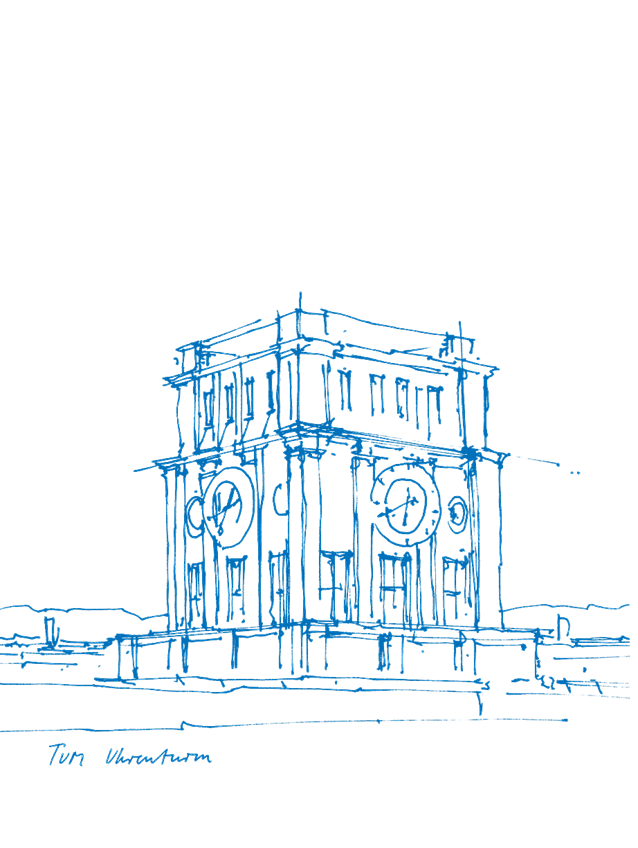
\includegraphics{img/TUM_Uhrenturm.png}%
    \end{textblock*}%
}

\newcommand{\PraesentationStartseiteUhrenturm}{
    \setbeamertemplate{title page}{%
        \PraesentationSeitenkopfInhalt{img/Universitaet_Logo_RGB.pdf}
        \PraesentationBildUhrenturm
        \PraesentationTitelseiteInhalt
    }
}

\newcommand{\PraesentationStartseiteLeer}{
    \setbeamertemplate{title page}{%
        \PraesentationSeitenkopfInhalt{img/Universitaet_Logo_weiss.pdf}
        \PraesentationTitelseiteInhalt
    }
}


\newcommand{\PraesentationMasterStandard}{
    \PraesentationFarbschemaStandard

    \PraesentationStartseiteUhrenturm

    \setbeamertemplate{headline}{
        \PraesentationSeitenkopfInhalt{img/Universitaet_Logo_RGB.pdf}
    }
}

\newcommand{\PraesentationMasterWeissBlau}{
    \PraesentationFarbschemaWeissBlau

    \PraesentationStartseiteLeer

    \setbeamertemplate{headline}{
        \PraesentationSeitenkopfInhalt{img/Universitaet_Logo_weiss.pdf}
    }
}

\newcommand{\PraesentationMasterKopfzeileDreizeiler}{
    \PraesentationFarbschemaStandard

    \setbeamertemplate{title page}{%
        \PraesentationBildUhrenturm
        \begin{textblock*}{\paperwidth}[0,0](0cm, -7.8mm)%
            \color{TUMBlau}\PraesentationSchriftgroesseDreizeiler\selectfont%
            \LehrstuhlName\\%
            \FakultaetName\\%
            \UniversitaetName\\%
            \normalcolor\normalsize\selectfont%
        \end{textblock*}%
        \PraesentationSeitenkopfInhalt{img/Universitaet_Logo_RGB.pdf}
        \PraesentationTitelseiteInhalt
    }

    \setbeamertemplate{headline}{
        \begin{textblock*}{\paperwidth}[0,0](0cm, -7.8mm)%
            \color{TUMBlau}\PraesentationSchriftgroesseDreizeiler\selectfont%
            \LehrstuhlName\\%
            \FakultaetName\\%
            \UniversitaetName\\%
            \normalcolor\normalsize\selectfont%
        \end{textblock*}%
        \PraesentationSeitenkopfInhalt{img/Universitaet_Logo_RGB.pdf}
    }
}

\newcommand{\PraesentationMasterWeissSchwarz}{
    \PraesentationFarbschemaWeissSchwarz

    \setbeamertemplate{title page}{%
        \PraesentationTitelseiteInhalt
        \PraesentationSeitenkopfInhalt{img/Universitaet_Logo_weiss.pdf}
    }

    \setbeamertemplate{headline}{
        \PraesentationSeitenkopfInhalt{img/Universitaet_Logo_weiss.pdf}
    }
}

\newcommand{\PraesentationTitelseite}{\frame[plain]{\titlepage}}
\newcommand{\PraesentationUeberschriftZweizeilig}[2]{\frametitle{#1\\[8mm]#2}}

\setbeamersize{
    text margin left=\PraesentationSeitenrand,
    text margin right=\PraesentationSeitenrand
}

\setbeamertemplate{frametitle}{%
    {\rule{0pt}{42mm + \PraesentationPositionKorrekturOben}\PraesentationSchriftgroesseSehrGross\selectfont\insertframetitle\newline\vspace*{-6.7mm}}%
}

% Aufzählungen:
\newcommand{\PraesentationAufzaehlungEbeneEinsSymbol}{\raise2pt\hbox{\donotcoloroutermaths\usebeamercolor{itemize subitem}\PraesentationSchriftgroesseAufzaehlungszeichen$\bullet$}}
\newcommand{\PraesentationAufzaehlungEbeneZweiSymbol}{\raise1.25pt\hbox{\donotcoloroutermaths\usebeamercolor{itemize subitem}$-$}}
\setbeamertemplate{itemize items}[circle]
\setbeamertemplate{itemize subitem}[triangle]
\setbeamercolor{itemize subitem}{fg=black}
\setbeamerfont{itemize/enumerate subbody}{size=\normalsize}
\setbeamertemplate{itemize item}{\PraesentationAufzaehlungEbeneEinsSymbol}
\setbeamertemplate{itemize subitem}{\PraesentationAufzaehlungEbeneZweiSymbol{}}
%\addtolength{\leftmarginii}{16mm-2pt}%

\newenvironment{PraesentationAufzaehlung}
{%
    \vspace{-\baselineskip}%
    \begin{itemize}%
        \setlength{\itemsep}{0pt}%
        \setlength{\parskip}{0pt}%
        \setlength{\parsep}{0pt}%
        \addtolength{\itemindent}{-1ex}%
}{%
    \end{itemize}%
}

%%%%%%%%%%%%%%%%%%%%%%%%%%%%%%%%%%%%%%%%%%%%%%%%%%%%%%%%%%%%%%%%%%%%%%%%%%%%%%%%
% DOKUMENT
%%%%%%%%%%%%%%%%%%%%%%%%%%%%%%%%%%%%%%%%%%%%%%%%%%%%%%%%%%%%%%%%%%%%%%%%%%%%%%%%


% PDF-Einstellungen:
\hypersetup{
    pdfstartview={Fit},
    pdfproducer={\AllgemeinErsteller},
    pdfcreator={\AllgemeinGestalter}
}

\textblockorigin{\PraesentationSeitenrand}{\PraesentationSeitenrand} % Ursprung für Positionierung

\setbeamerfont{footnote}{size=\PraesentationSchriftgroesseKlein}

\setbeamertemplate{footline}{
    \hbox{%
        \usebeamerfont{footnote}%
        \begin{beamercolorbox}[wd=.9\paperwidth]{}%
            \hspace*{\PraesentationSeitenrand}%
            \PraesentationFusszeileZusatz{}%
        \end{beamercolorbox}%
        \begin{beamercolorbox}[wd=.1\paperwidth]{}%
            \insertframenumber{}%
            \raggedleft
            \hspace*{\PraesentationSeitenrand}%
        \end{beamercolorbox}%
        \vspace*{3.25mm}%
    }%
}

\setbeamertemplate{navigation symbols}{}

\begin{document}
\setlength{\baselineskip}{\PraesentationAbstandAbsatz}
\setlength{\parskip}{\baselineskip}
 % !!! NICHT ENTFERNEN !!!
%%%%%%%%%%%%%%%%%%%%%%%%%%%%%%%%%%%%%%%%%%%%%%%%%%%%%%%%%%%%%%%%%%%%%%%%%%%%%%%%


%%%%%%%%%%%%%%%%%%%%%%%%%%%%%%%%%%%%%%%%%%%%%%%%%%%%%%%%%%%%%%%%%%%%%%%%%%%%%%%%
% FOLIENSTIL: Standard
\PraesentationMasterStandard

\PraesentationTitelseite % Fügt die Startseite ein


% draws an arrow from (#2,#3) to (#2+#4,#3) with height of #5 (arrow in x direction)
% color (and other arguments, like visible on), startX, startY, length (X dir), height (Y dir)
\newcommand{\TikZArrowX}[5]{
    \filldraw[#1] (#2,#3) -- (#2,#3+#5*2/3) -- (#2+#4/2,#3+#5*2/3) -- (#2+#4/2,#3+#5) -- (#2+#4,#3) -- (#2+#4/2,#3-#5) -- (#2+#4/2,#3-#5*2/3) -- (#2,#3-#5*2/3) -- (#2,#3);
    \draw[#1, black] (#2,#3) -- (#2,#3+#5*2/3) -- (#2+#4/2,#3+#5*2/3) -- (#2+#4/2,#3+#5) -- (#2+#4,#3) -- (#2+#4/2,#3-#5) -- (#2+#4/2,#3-#5*2/3) -- (#2,#3-#5*2/3) -- (#2,#3);
}

% draws an arrow from #2,#3) to (#2,#3+#5) with height of #4 (arrow in y direction)
% color (and other arguments, like visible on), startX, startY, length (X dir), height (Y dir), color
\newcommand{\TikZArrowY}[5]{
    \filldraw[#1] (#2,#3) -- (#2+#4*2/3,#3) -- (#2+#4*2/3,#3+#5/2) -- (#2+#4,#3+#5/2) -- (#2,#3+#5) -- (#2-#4,#3+#5/2) -- (#2-#4*2/3,#3+#5/2) -- (#2-#4*2/3,#3) -- (#2,#3);
    \draw[#1, black] (#2,#3) -- (#2+#4*2/3,#3) -- (#2+#4*2/3,#3+#5/2) -- (#2+#4,#3+#5/2) -- (#2,#3+#5) -- (#2-#4,#3+#5/2) -- (#2-#4*2/3,#3+#5/2) -- (#2-#4*2/3,#3) -- (#2,#3);
}

% draws one entry of the color legend for the program scheme
% color, text, posX, posY (left, top coordinate)
\newcommand{\colorLegendEntry}[4]{
    \filldraw[#1] (#3,#4) rectangle (#3+1,#4+1);
    \draw[black] (#3,#4) rectangle (#3+1,#4+1);
    \node at (#3+0.5,#4+0.4) (color_legend_entry_point) {};
    \node[right=2mm of color_legend_entry_point] (color_legend_entry_text) {#2};
}

% draws a color legend for the program scheme
% posX, posY (left, top coordinate)
\newcommand{\colorLegend}[2] {
    \colorLegendEntry{TUMOrange}{Static Translator Parts}{#1}{#2}
    \colorLegendEntry{TUMBlauDunkel}{Intermediate Representation (IR)}{#1}{#2-1.5}
    \colorLegendEntry{purple}{Maschine Code / ELF File}{#1}{#2-3}
}

% draws the schematic presentation of the program
% scale, fontSize
\newcommand{\ProgramSchemeVersionOne}[2]{
    \begin{center}
        \begin{tikzpicture}[very thick, scale=#1]
            % draw color legend
            \colorLegend{-2}{-6}

            % riscv elf file rectangle
            % background
            \filldraw[purple] (-2,-2) rectangle (2,2);
            % black border
            \draw[black] (-2,-2) rectangle (2,2);
            % label
            \node[align=center, color=white] at (0,0) (riscv_text) {\fontsize{#2}{#2} \selectfont RISC-V};

            % lifter arrow
            \TikZArrowX{TUMOrange}{2}{0}{6}{1.5}
            % arrow label
            \node[align=center, color=white] at (4.5,0) (lifter_text) {\fontsize{#2}{#2} \selectfont Lifter};

            % ir (unoptimized) rectangle
            % background
            \filldraw[TUMBlauDunkel] (8,-2) rectangle (12,2);
            % black border
            \draw[black] (8,-2) rectangle (12,2);
            % label
            \node[align=center, color=white] at (10,0) (ir_text_1) {\fontsize{#2}{#2} \selectfont IR};

            % optimizer arrow
            \TikZArrowX{TUMOrange}{12}{0}{6}{1.5}
            % arrow label
            \node[align=center, color=white] at (14.5,0) (optimizer_text) {\fontsize{#2}{#2} \selectfont Optimizer};

            % ir (optimized) rectangle
            % background
            \filldraw[TUMBlauDunkel] (18,-2) rectangle (22,2);
            % black border
            \draw[black] (18,-2) rectangle (22, 2);
            % label
            \node[align=center, color=white] at (20,0) (ir_text_2) {\fontsize{#2}{#2} \selectfont IR};

            % compiler arrow
            \TikZArrowX{TUMOrange}{22}{0}{6}{1.5}
            % arrow label
            \node[align=center, color=white] at (24.5,0) (generator_text) {\fontsize{#2}{#2} \selectfont Generator};

            % x86_64 rectangle
            %background
            \filldraw[purple] (28,-2) rectangle (32,2);
            % black border
            \draw[black] (28,-2) rectangle (32,2);
            % label
            \node[align=center, color=white] at (30,0) (x86_64_text) {\fontsize{#2}{#2} \selectfont x86\_64};
        \end{tikzpicture}
    \end{center}
}

%%%%%%%%%%%%
%% Inhalt %%
%%%%%%%%%%%%

\begin{frame}
    \frametitle{Inhalt}
    \begin{itemize}
        \item
    \end{itemize}
\end{frame}

%%%%%%%%%%%%%%%%%%%%%%%
%% Programmübersicht %%
%%%%%%%%%%%%%%%%%%%%%%%

\begin{frame}
    \frametitle{Programmübersicht}
    \note[item]{Ziel: Statische Binärübersetzung}
    \note[item]{Übersetzung von Binärdateien auf eine andere Plattform}
    \note[item]{Dynamisch wäre ein Interpreter, also zur Laufzeit, bei uns Übersetzung zur Compilezeit}
    \note[item]{hier: von RISC-V zu x86\_64}
    \note[item]{RISC, feste 32-Bit Befehlslänge}
    \note[item]{wenige, einfache Befehle -> geringe Codedichte, aber leicht zu übersetzten}
    \note[item]{Register-Register-Maschine, also nur Operation auf Registern in der Dreioperandenform, s. 'ERA'}
    \note[item]{Lifter 'hebt' RISC-V in die Zwischenrepräsentation (sog. IR)}
    \note[item]{Optimierung auf der IR: aktuell noch Identitätsbbildung}
    \note[item]{Compiler compiliert zu Assemlby Code und dieser wird zu einer ausführbaren Datei assembliert}

    %alignment to have some space between headline an the schematic
    ~\\
    ~\\
    \ProgramSchemeVersionOne{0.6}{18}
\end{frame}

%%%%%%%%%%%%%%%%%%%%%
%% IR Aufbau Folie %%
%%%%%%%%%%%%%%%%%%%%%

\begin{frame}
    \frametitle{Intermediate Representation}{Aufbau}
    \note[item]{Selbst definierte Zwischenrepräsentation}
    \note[item]{Hauptbestandteil: Basic Blocks}
    \note[item]{-> Sequentielle Folge von Instruktionen, die durch Kontrollflussoperation beendet werden}
    \note[item]{Basic Block enthält Variablen in sogenannter SSA-Form und die dazu gehörenden Operationen}
    \note[item]{Static single assignment -> Jeder var wird nur einmal Wert zugewiesen}
    \note[item]{-> Vereinfacht Optimierungen}
    \note[item]{Eingaben kommen als "Statics" -> Abstrakte Darstellung von RISCV-Registern}
    \note[item]{Kontrollflussoperationen verbinden die Basic Blocks}
    \note[item]{SSA bedeutet: Variablen frei verschiebbar, deshalb Memory Tokens für Einhaltung der Reihenfolge}
    \pause{}
    \begin{itemize}
        \item Programm aus \textbf{Basic Blocks}
        \item \textbf{Static Single Assignment (SSA)}
        \item Eingaben in Form von Statics
        \item Verbindung durch Kontrollflussoperationen
    \end{itemize}
\end{frame}

\begin{frame}
    \frametitle{Intermediate Representation}{Operationen}

    ~\\
    ~\\

    \begin{columns}[c]
        \column{0.4\textwidth}
        Instruktionen:
        \begin{itemize}
            \item Speicher: \texttt{store}, \texttt{load}
            \item Arithmetisch: \texttt{add}, \texttt{sub}, \texttt{mul}, ...
            \item Logisch: \texttt{and}, \texttt{or}, \texttt{shl}, ...
            \item Sonstige: Typkonvertierung, ...
        \end{itemize}

        \column{0.4\textwidth}
        Kontrollflussoperationen:
        \begin{itemize}
            \item Sprünge: \texttt{jump}, \texttt{ijump}, \texttt{cjump}
            \item \texttt{unreachable}
            \item \texttt{syscall}
        \end{itemize}
    \end{columns}
\end{frame}

%%%%%%%%%%%%%%
%% IR Folie %%
%%%%%%%%%%%%%%

\begin{frame}[fragile]
    \frametitle{Intermediate Representation}{Beispiel}
    \pause{}
    ~\\
    ~\\
    ~\\
    \begin{columns}[c]
        \column{0.275 \textwidth}
        \begin{lstlisting}[language=rv64]
        [...]
        addi a0, x0, 100
        j somewhere_else
        [...]
        \end{lstlisting}

        \column{0.125 \textwidth}
        \begin{tikzpicture}[scale=0.72]
            \TikZArrowX{TUMOrange}{0}{0}{4}{1}
        \end{tikzpicture}


        \column{0.6 \textwidth}
        \begin{lstlisting}[language=SbtIr]
block b1(/* inputs */) <= [/* predecessors */] {
    imm v32 <- immediate 0
    imm v33 <- immediate 100
    i64 v34 <- add imm v32, imm v33
} => [(jump, [b2, i64 v34])]
    \end{lstlisting}
    \end{columns}

\end{frame}
\clearpage

%%%%%%%%%%%%%%%%%%%%%%%%%%%
%% ELF File Parser Folie %%
%%%%%%%%%%%%%%%%%%%%%%%%%%%

\begin{frame}[fragile]
    \frametitle{Lifter}{ELF Binärdatei laden und Instruktionsbytes decodieren}
    \begin{enumerate}
        \setlength\itemsep{0.6em}
              \note[item]{ELF Prüfung: Prüfbits, System-V ABI, 64-Bit, Little Endian, RISC-V Machine}
        \item ELF File prüfen.
              \note[item]{Symbole weren bei gestrippten ELF-Binaries nicht eingelesen}
        \item Program Header, Sections und Symbole auslesen.
              \note[item]{32-Byte bzw. 16-Byte Compressed mit frvdec decodieren}
              \vspace{0.5em}
              \begin{enumerate}
                  \setlength\itemsep{0.6em}
                  \item Instruktionen aus \texttt{PROGBITS} Sektionen die \textit{ausführbar} sind \\
                        $\rightarrow$ mit \textbf{frvdec} decodieren.
                  \item Daten aus \textit{lesbaren} Sektionen die \textbf{nicht} \textit{ausführbar} sind
              \end{enumerate}
    \end{enumerate}
\end{frame}
\clearpage

%%%%%%%%%%%%%%%%%%%%%%%%%%
%% Lifter General Folie %%
%%%%%%%%%%%%%%%%%%%%%%%%%%

\begin{frame}
    \frametitle{Lifter}{RISC-V Instruktionen sequentiell in IR Code umwandeln}\\
    Wiederhole solange ungeliftete Instruktionen existieren:
    \begin{enumerate}
        \setlength{\itemsep}{1em}
        \item Starte neuen Basic Block bei der nächsten, ungelifteten Instruktion
        \item geladene Instruktionen in IR parsen
        \item Wiederhole solange bis:
              \begin{enumerate}
                  \vspace{1em}
                  \setlength{\itemsep}{1em}
                  \item eine \textbf{Kontrollfluss ändernde Instruktion} auftritt
                  \item der Start eines
                        neues Basic Blocks an der nächsten Instruktion registriert ist
              \end{enumerate}
        \item Beende Basic Block $\rightarrow$ markiere Start neuer Basic Blöcke an evtl. Sprungzielen
    \end{enumerate}
\end{frame}
\clearpage

%%%%%%%%%%%%%%%%%%%%%%
%% Lifter Splitting %%
%%%%%%%%%%%%%%%%%%%%%%
\begin{frame}
    \frametitle{Lifter Splitting}{Aufteilen eines Basic Blocks}
    \begin{itemize}
        \setlength{\itemsep}{1em}
        \item Situation: Sprung \textbf{in} einen Basic Block
        \item Aufteilung an Sprungadresse in zwei Basic Blöcke
        \item Verbindung mit einem direkten Sprung
        \item Komplexe Operation, da alle Referenzen auf den geteilten Block betrachtet werden müssen
    \end{itemize}
\end{frame}
\clearpage

%%%%%%%%%%%%%%%%%%%%%%%%%
%% Lifter Backtracking %%
%%%%%%%%%%%%%%%%%%%%%%%%%

\begin{frame}
    \frametitle{Lifter Backtracking}{Rücklverfolgung einer indirekten Sprungadresse}\\
    = rekursive Rückverfolgung der absoluten Werte aller Operationsparameter
    \begin{figure}
        \centering
        \begin{tikzpicture}[scale=1.5]
            \begin{pgfonlayer}{nodelayer}
                \node [style=BB] (0) at (-3.75, 0) {bb24};
                \node [style=VAR] (1) at (-2.25, 0) {v37};
                \node [style=OP] (2) at (-0.75, 0) {ADD};
                \node [style=VAR] (3) at (0.5, 1.5) {v36};
                \node [style=VAR] (4) at (0.5, -1.5) {v34};
                \node [style=OP] (5) at (2, -1.5) {SHL};
                \node [style=VAR] (6) at (3.5, 0.25) {v15};
                \node [style=VAR] (7) at (3.5, -1.5) {v22};
                \node [style=STATIC] (8) at (5, 0.25) {x14};
                \node [style=STATIC] (9) at (5, -1.5) {x21};
                \node [style=BB] (10) at (6.5, 1) {bb42};
                \node [style=BB] (11) at (6.5, -1) {bb23};
                \node [style=BB] (12) at (6.5, 2) {bb8};
                \node [style=BB] (13) at (6.5, 0) {bb17};
                \node [style=BB] (14) at (6.5, -2.25) {bb127};
                \node [style=VALUE] (15) at (2, 1.5) {-2};
                \node [style=VAR] (16) at (7.75, 2) {};
                \node [style=VAR] (18) at (7.75, 0) {};
                \node [style=VAR] (19) at (7.75, -1) {};
                \node [style=BB] (23) at (9.75, 1) {};
                \node [style=BB] (24) at (9.75, -2.25) {};
                \node [style=OP] (25) at (8.75, 0) {};
                \node [style=OP] (26) at (8.75, -1) {};
                \node [style=OP] (28) at (8.75, 2) {};
                \node [style=VAR] (29) at (7.75, 1) {};
                \node [style=VAR] (31) at (7.75, -2.25) {};
                \node [style=STATIC] (32) at (8.75, 1) {};
                \node [style=STATIC] (33) at (8.75, -2.25) {};
                \node [style=none] (34) at (9.75, 2) {};
                \node [style=none] (35) at (9.75, 1.5) {};
                \node [style=none] (36) at (9.75, 0.25) {};
                \node [style=none] (37) at (9.75, -0.25) {};
                \node [style=none] (38) at (9.75, -0.75) {};
                \node [style=none] (39) at (9.75, -1.25) {};
                \node [style=none] (40) at (9.75, 2.5) {};
            \end{pgfonlayer}
            \begin{pgfonlayer}{edgelayer}
                \draw [style=LINK] (0) to (1);
                \draw [style=LINK] (1) to (2);
                \draw [style=LINK] (2) to (3);
                \draw [style=LINK] (2) to (4);
                \draw [style=LINK] (3) to (15.center);
                \draw [style=LINK] (4) to (5);
                \draw [style=LINK] (5) to (7);
                \draw [style=LINK] (5) to (6);
                \draw [style=LINK] (6) to (8);
                \draw [style=LINK] (7) to (9);
                \draw [style=LINK] (9) to (14);
                \draw [style=LINK] (9) to (11);
                \draw [style=LINK] (8) to (13);
                \draw [style=LINK] (8) to (10);
                \draw [style=LINK] (8) to (12);
                \draw [style=LINK] (12) to (16);
                \draw [style=LINK] (13) to (18);
                \draw [style=LINK] (11) to (19);
                \draw [style=LINK] (16) to (28);
                \draw [style=LINK] (10) to (29);
                \draw [style=LINK] (29) to (32);
                \draw [style=LINK] (18) to (25);
                \draw [style=LINK] (14) to (31);
                \draw [style=LINK] (31) to (33);
                \draw [style=LINK] (33) to (24);
                \draw [style=LINK] (19) to (26);
                \draw [style=LINK] (32) to (23);
                \draw [style=DASHED] (28) to (34.center);
                \draw [style=DASHED] (28) to (35.center);
                \draw [style=DASHED] (25) to (36.center);
                \draw [style=DASHED] (25) to (37.center);
                \draw [style=DASHED] (26) to (38.center);
                \draw [style=DASHED] (26) to (39.center);
                \draw [style=DASHED] (28) to (40.center);
            \end{pgfonlayer}
        \end{tikzpicture}
    \end{figure}
\end{frame}
\clearpage

%%%%%%%%%%%%%%%%%%%%%%
%% Lifter Call / Return %%
%%%%%%%%%%%%%%%%%%%%%%
\begin{frame}
    \frametitle{Lifter Subroutinen}{Erkennung der Assembler Pseudoinstruktionen \texttt{call} und \texttt{ret}.}
    \begin{itemize}
        \setlength{\itemsep}{1em}
        \item RISC-V Subroutinen Aufrufe funktionieren anders als bei x86\_64
        \item Standard Calling Convention definiert \texttt{x1} und \texttt{x5} als \textit{Linkregister}
        \item \texttt{JAL} := \textit{Jump and Link}
        \item \texttt{JAL (x1 | x5), ..., ...} $\equiv$ \texttt{call}
        \item \texttt{JALR x0, x1, 0} $\equiv$ \texttt{ret}
        \item Laufzeitüberprüfung der Rücksprungziele durch Returnadressen-Stack 
    \end{itemize}
\end{frame}
\clearpage

%%%%%%%%%%%%%%%%%%%%%
%% Generator Folie %%
%%%%%%%%%%%%%%%%%%%%%

\begin{frame}
    \note[item]{Sehr einfache, aber korrekte Übersetztung}
    \note[item]{Originales ELF-Programm als binäres Speicherbild an exakter Adresse eingebunden}
    \note[item]{RISC-V System-V ABI (Startup, Syscall) zur Laufzeit emuliert}
    \note[item]{Stack wird nur initialisiert, danach nicht mehr im Generator speziell behandelt}
    \note[item]{Indirekte Sprünge werden per Lookup zur Laufzeit aufgelöst}
    %    \note[item]{Erste Optimierung: Eliminierung von Redundanzen bei den Statics}

    \frametitle{Generator}{Übersetztung der IR zu x86\_64}
    \begin{itemize}
        \setlength{\itemsep}{1em}
        \item Sehr einfache, aber korrekte Übersetztung
        \item Originales ELF-Programm als binäres Speicherbild an exakter Adresse eingebunden
              %        \item Stellt nur initialen Stack zur Verfügung % es wird nicht der x86-64 Stack verwendet
        \item RISC-V System-V ABI (Startup, Syscall) zur Laufzeit emuliert
        \item Indirekte Sprünge werden per Lookup zur Laufzeit aufgelöst
        \item Erste Optimierung: Eliminierung von Redundanzen bei den Statics
    \end{itemize}
\end{frame}
\clearpage

%%%%%%%%%%%%%%%%%%%
%% IJump hashing %%
%%%%%%%%%%%%%%%%%%%

\begin{frame}
    \frametitle{Basic Block Startadressen}{Datenstruktur für effizienten Zugriff auf Basic Block Startadressen}
    \vspace{1cm}
    \begin{columns}[t]
        \column{0.55 \textwidth}
        \textbf{Naive Implementierung}
        \begin{itemize}
            \vspace{1em}
            \setlength{\itemsep}{1em}
            \item Speichere für jede RISC-V Instruktion die korrespondierende Basic Block Startadresse
            \item Wenn diese nicht existiert, füge stattdessen 0 ein
            \item Liste dieser Wert baut Adressraum der originalen Binary nach
        \end{itemize}
        \column{0.45 \textwidth}
        \textbf{Fast perfektes Hashing}
        \begin{itemize}
            \vspace{1em}
            \setlength{\itemsep}{1em}
            \item Ordne Startadressen in Hashtabelle ein
            \item Zweistufiges hashing durch Einsortieren in Buckets
            \item ``Hash, Displace, and Compress''-Verfahren gepaart mit der SpookyHash Funktion
        \end{itemize}
    \end{columns}
\end{frame}
\clearpage

\begin{frame}
    \frametitle{Basic Block Startadressen}{Vorteile und Nachteile}
    \vspace{1cm}
    \begin{columns}[t]
        \column{0.55 \textwidth}
        \textbf{Naive Implementierung}
        \begin{itemize}
            \vspace{1em}
            \setlength{\itemsep}{1em}
            \item Zugriffszeit in $O(1)$
            \item Adresszugriff benötigt \textbf{eine} Ladeoperation
            \item Benötigt genau so viel Speicher wie der geliftete Teil der originalen Binary
        \end{itemize}
        \column{0.45 \textwidth}
        \textbf{Fast perfektes Hashing}
        \begin{itemize}
            \vspace{1em}
            \setlength{\itemsep}{1em}
            \item Zugriffszeit in $O(1)$
            \item Runtime Overhead: Hashtabellenindex muss zur Laufzeit berechnet werden
            \item Benötigter Speicherplatz in $O(n)$ mit $n = \text{Anzahl der Startadressen}$
        \end{itemize}
    \end{columns}
\end{frame}
\clearpage


%%%%%%%%%%%%%%%%%%%%%%%%%%%%%%
%% Technische Demonstration %%
%%%%%%%%%%%%%%%%%%%%%%%%%%%%%%

\begin{frame}[fragile]
    \frametitle{Technische Demonstration}{Live Demonstration des aktuellen Standes}

    % Dauer: ~3m
    \note[item]{Kompilieren zu RISCV-64 mit einer unmodifizierten musl libc (standardbibliothek)}
    \note[item]{Unser Program übersetzt zu x86 assembly + binary image}
    \note[item]{Assemblieren mittels GNU tools}
    \note[item]{Linken von binary image, übersetztem assembly und hilfsbibliothek}
    \note[item]{Ausführen}
    \note[item]{Ausführen, ungefährere Vergleich (native, qemu, translated) => Wo sind wir mit optimierungen, fast faktor 10 langsamer als QEMU}

    % Setup:
    % Use xfc4, configure beamer as display to the right
    % Go To Workspace 1, start pympress with
    % LC_ALL=de_DE.UTF-8 pympress presentation/build/presentation_16_9.pdf
    % Go To Workspace 2, on laptop start xfce4-terminal with
    % 1. Open new Terminal Window on laptop with `tmux new-session -s demo -A`
    % 2. Open new Terminal Window on presentation screen with `tmux attach-session -r -t demo`
    % Resize as necessary (ctrl + + or -)
    %
    % Commands:
    % ./big_tests/sysroot/bin/riscv64-linux-gnu-gcc -static examples/helloworld3.c -o examples/helloworld3
    %
    % ./build/src/translate --debug=true --print-ir=true --output-binary=examples/helloworld3.bin --output=examples/helloworld3_translated.s examples/helloworld3
    % gcc -c examples/helloworld3_translated.s -o examples/helloworld3_translated.o
    % ld -T src/generator/x86_64/helper/link.ld examples/helloworld3_translated.o build/src/generator/x86_64/helper/libhelper.a -o examples/helloworld3_translated
    %
    % ./examples/helloworld3_translated
    %
    % Additional:
    % gcc examples/helloworld3.c -o examples/helloworld3_native
    % time ./examples/helloworld3_native
    % time ./examples/helloworld3
    % time ./examples/helloworld3_translated
    \begin{columns}[c]
        \column{0.50 \textwidth}
        \begin{lstlisting}[language=bash, basicstyle=\small\ttfamily, extendedchars=true,escapeinside={@@}]
./big_tests/sysroot/bin/riscv64-linux-gnu-gcc \
    -static \
    examples/helloworld3.c \
    -o examples/helloworld3

./build/src/translate \
    @-@-debug=true \
    @-@-output-binary=examples/helloworld3.bin \
    @-@-output=examples/helloworld3_translated.s \
    examples/helloworld3
    \end{lstlisting}

        \column{0.5 \textwidth}
        \begin{lstlisting}[language=bash, basicstyle=\small\ttfamily, extendedchars=true,escapeinside={@@}]
gcc \
    -c examples/helloworld3_translated.s \
    -o examples/helloworld3_translated.o

ld \
    -T src/generator/x86_64/helper/link.ld \
    examples/helloworld3_translated.o \
    build/src/generator/x86_64/helper/libhelper.a \
    -o examples/helloworld3_translated

./examples/helloworld3_translated
    \end{lstlisting}
    \end{columns}
\end{frame}
\clearpage

%%%%%%%%%%%%%%%%%%%%%
%% Erreichte Ziele %%
%%%%%%%%%%%%%%%%%%%%%

\begin{frame}
    \frametitle{Erreichte Ziele}{Erreichte Hauptziele und Ausblick}

    % Dauer: mind. 1 Minute, ansonsten flexible
    \note[item]{Freistehend => ohne standard bibliothek, z\.B\. handgeschriebenes assembly oder einfache C programme}
    \note[item]{Atomics werden nur also nicht atomics übersetzt so weit nötig}
    \note[item]{Demonstriert im Beispiel}
    \note[item]{2 Bugs in musl libc, malloc, fehlender BasicBlock in printf\_core wegen switch statement ohne control fluss änderung am ende von cases}
    \note[item]{Und noch vereinzelt weiter instructionen je nach bedarf}
    \note[item]{ijump eigentlich bei erweiterte Ziele, aber extrem wichtig da für return verwendet}

    \begin{itemize}
        \item Korrektes Übersetzen einfacher freistehender Programme
        \item Übersetzen von unmodifizierter musl libc
        \item Unterstützung von RV64I, RV64C, \ldots{}
        \item Auflösung indirekter Sprünge zur Laufzeit
    \end{itemize}
\end{frame}

%%%%%%%%%%%%%%%%%%%
%% Noch Fragen ? %%
%%%%%%%%%%%%%%%%%%%

\begin{frame}
    \frametitle{Noch Fragen?}{}
\end{frame}

%%%%%%%%%%%%%%%%%%%%%%%%%
%% Generator-Translate %%
%%%%%%%%%%%%%%%%%%%%%%%%%

\begin{frame}[fragile]
    \frametitle{Generator}
    \begin{columns}[c]
        \column{0.45 \textwidth}
        \begin{lstlisting}[language=SbtIr, escapechar=!]
        block b1(/* inputs */) <= [/* predecessors */] {
            !\only<1|handout:0>{\colorbox{yellow}{i64 v0 <- @1}}!!\alt<1>{}{\colorbox{white}{i64 v0 <- @1}}!
            !\only<2|handout:0>{\colorbox{yellow}{imm v1 <- immediate 0}}!!\alt<2>{}{\colorbox{white}{imm v1 <- immediate 0}}!
            !\only<3|handout:0>{\colorbox{yellow}{imm v2 <- immediate 100}}!!\alt<3>{}{\colorbox{white}{imm v2 <- immediate 100}}!
            !\only<4|handout:0>{\colorbox{yellow}{i64 v3 <- add i64 v1, i64 v2}}!!\alt<4>{}{\colorbox{white}{i64 v3 <- add i64 v1, i64 v2}}!
        } => [!\only<5|handout:0>{\colorbox{yellow}{(jump, [b2, i64 v34])}}!!\alt<5>{}{\colorbox{white}{(jump, [b2, i64 v34])}}!]
    \end{lstlisting}

        \column{0.125 \textwidth}
        \begin{tikzpicture}[scale=0.72]
            \TikZArrowX{TUMOrange}{0}{0}{4}{1}
        \end{tikzpicture}

        \column{0.35 \textwidth}
        \begin{lstlisting}[language=rv64, escapechar=!]
b1:
!\colorbox{white}{push rbp}!
!\colorbox{white}{mov rbp, rsp}!
!\colorbox{white}{sub rsp, 32}!
!\only<1|handout:0>{\colorbox{yellow}{mov rax, [s0]}}!!\alt<1>{}{\colorbox{white}{mov rax, [s0]}}!
!\only<1|handout:0>{\colorbox{yellow}{mov [rbp - 8 * 1], rax}}!!\alt<1>{}{\colorbox{white}{mov [rbp - 8 * 1], rax}}!
!\only<2|handout:0>{\colorbox{yellow}{mov [rbp - 8 * 2], 0}}!!\alt<2>{}{\colorbox{white}{mov [rbp - 8 * 2], 0}}!
!\only<3|handout:0>{\colorbox{yellow}{mov [rbp - 8 * 3], 100}}!!\alt<3>{}{\colorbox{white}{mov [rbp - 8 * 3], 100}}!
!\only<4|handout:0>{\colorbox{yellow}{mov rax, [rbp - 8 * 2]}}!!\alt<4>{}{\colorbox{white}{mov rax, [rbp - 8 * 2]}}!
!\only<4|handout:0>{\colorbox{yellow}{mov rbx, [rbp - 8 * 3]}}!!\alt<4>{}{\colorbox{white}{mov rbx, [rbp - 8 * 3]}}!
!\only<4|handout:0>{\colorbox{yellow}{add rax, rbx}}!!\alt<4>{}{\colorbox{white}{add rax, rbx}}!
!\only<4|handout:0>{\colorbox{yellow}{mov [rbp - 8 * 4], rax}}!!\alt<4>{}{\colorbox{white}{mov [rbp - 8 * 4], rax}}!
!\only<5|handout:0>{\colorbox{yellow}{mov rax, [rbp - 8 * 4]}}!!\alt<5>{}{\colorbox{white}{mov rax, [rbp - 8 * 4]}}!
!\only<5|handout:0>{\colorbox{yellow}{mov [s0], rax}}!!\alt<5>{}{\colorbox{white}{mov [s0], rax}}!
!\only<5|handout:0>{\colorbox{yellow}{jmp b2}}!!\alt<5>{}{\colorbox{white}{jmp b2}}!
        [...]
        \end{lstlisting}

    \end{columns}

\end{frame}
\clearpage

%%%%%%%%%%%%%%%%%%%%%%%%%%%%%%%%%%%%
%% Split Basic Block Backup Folie %%
%%%%%%%%%%%%%%%%%%%%%%%%%%%%%%%%%%%%

\begin{frame}[fragile]
    \frametitle{Basic Block Splitting}{Beispiel}
    ~\\
    ~\\
    ~\\
    \begin{columns}[c]
        \column{0.275 \textwidth}
        \begin{lstlisting}[language=rv64]
        [...]
        addi a1, x0, 100
    loop:
        addi a1, a1, -1
        bne a1, x0, loop
        [...]
        \end{lstlisting}

        \column{0.125 \textwidth}
        \begin{tikzpicture}[scale=0.72]
            \TikZArrowX{TUMOrange}{0}{0}{4}{1}
        \end{tikzpicture}

        \column{0.6 \textwidth}
        \begin{lstlisting}[language=SbtIr]
block b1(inputs) <= [predecessors] {
    i64 v0 <- @1
    [...] // more statics
    imm v33 <- immediate 0
    imm v34 <- immediate 100
    i64 <- add i64 v33, i64 v33
    [...]
} => [(jump, [b2, ...])]

block b2(inputs) <= [predecessors] { // loop
    [...] // statics
    imm v33 <- immediate -1
    i64 v34 <- add i64 v11, i64 v33
    [...]
} => [(cjump, [b2, ...]), (jump, [...])]
    \end{lstlisting}
    \end{columns}

\end{frame}
\clearpage

%%%%%%%%%%%%%%%%%%%%%%%%%%%%%%%%%%%%%%%%%%%%%%%%%%%%%%%%%%%%%%%%%%%%%%%%%%%%%%%%
\end{document} % !!! NICHT ENTFERNEN !!!
%%%%%%%%%%%%%%%%%%%%%%%%%%%%%%%%%%%%%%%%%%%%%%%%%%%%%%%%%%%%%%%%%%%%%%%%%%%%%%%%
